\documentclass[conference]{IEEEtran}

\usepackage{amsmath,amssymb}
\usepackage{graphicx}
\usepackage{booktabs}
\usepackage{algorithm}
\usepackage{algpseudocode}
\usepackage{url}

\title{RiskShield-Hierarchical HRMPPO-MPC: Causal Hierarchical Safe Reinforcement Learning for Construction-Site Inspection under Perception Uncertainty}
\author{\IEEEauthorblockN{Mahmoud Maher}}

\begin{document}
\maketitle

\begin{abstract}
Autonomous construction inspection couples sparse coverage objectives with
collisions, worker proximity, restricted areas, and imperfect visual
perception. We present a reproducible Gymnasium benchmark, RiskShield-PPO
(PPO-Lagrangian with an auxiliary cost-value estimator), and a predictive
action shield. A five-algorithm matrix evaluates 1,350 episodes over three site
sizes, three hazard densities, three perception-noise levels, and ten paired
seeds; six ablations add 180 episodes. RiskShield-PPO reduced mean safety cost
from PPO's 49.39 to 17.13 and eliminated observed collisions, but neither
learned method completed a full mission. Frontier exploration achieved 96.67\%
success and 0.998 hazard recall, exposing a substantial learning gap. A
separate Webots runtime verifies CUDA perception, shielded policy-to-motor
control, and rendered Webots operation. The project also evaluates an
experimental hierarchical v4 policy on 270
paired held-out grid episodes. It achieved 58.89\% mission success and
92.14\% hazard recall in that protocol; production remains RiskShield-PPO v1
because the v4 replacement gates were rejected. The evidence is simulation-only
and does not establish real-world safety.
\end{abstract}

\section{Introduction}
Construction inspection requires visiting hazards while avoiding workers,
restricted regions, machinery, and fall risks. Reward maximization alone does
not express an acceptable risk budget, and perception errors make fixed safety
assumptions unreliable. Safe RL commonly modifies the objective or constrains
exploration \cite{garcia2015safe}; constrained policy optimization formalizes
cost limits \cite{achiam2017cpo}, while shields can replace actions before
execution \cite{alshiekh2018shielding}.

This project contributes (i) a typed, deterministic construction-inspection
benchmark; (ii) genuine PPO, SAC, planner, and constrained baselines; (iii)
RiskShield-PPO and a separable $k$-step shield; (iv) controlled perception
uncertainty; and (v) an integrated Webots demonstration. We make no claim of
learned-policy task mastery: the complete matrix shows zero mission success
for all three learned policies.

\section{Related Work}
PPO optimizes a clipped policy-ratio surrogate \cite{schulman2017ppo}. SAC is
an off-policy maximum-entropy actor--critic method \cite{haarnoja2018sac}.
CMDP methods optimize reward subject to expected cost \cite{achiam2017cpo}.
Shielding instead filters proposed actions with an external safety model
\cite{alshiekh2018shielding}. Our system combines a Lagrangian training signal
with a predictive runtime filter; it does not inherit formal guarantees from
either cited method. Gymnasium provides the standardized environment API
\cite{towers2024gymnasium}, and Webots supplies the robot simulator
\cite{michel2004webots}.

\section{Problem Formulation}
We model a finite-horizon CMDP
$\mathcal{M}=(\mathcal{S},\mathcal{A},P,r,c,\gamma,d)$.
The discrete actions are north, south, west, east, and inspect. The observation
contains padded semantic map channels (obstacle, hazard, worker, restricted,
visited, agent, risk, dynamic hazard, PPE risk, visibility), pose,
orientation, progress, local risk, and an action mask.

Reward separates task progress from cost:
\begin{equation}
r_t=-0.01+r_{\mathrm{inspect}}+r_{\mathrm{coverage}}-r_{\mathrm{invalid}},
\end{equation}
while
\begin{equation}
c_t=c_{\mathrm{collision}}+c_{\mathrm{near}}+
c_{\mathrm{restricted}}+c_{\mathrm{PPE}}.
\end{equation}
The objective is
\begin{equation}
\max_\pi J_R(\pi)\quad\mathrm{s.t.}\quad J_C(\pi)\le d,
\end{equation}
with training budget $d=5$. Reward and cost remain separately logged.

\section{Construction Safety RL Benchmark}
Three parameterized grid sites vary size, hazards, workers, dynamic obstacles,
and episode horizon. Reset and transition randomness use explicit seeds.
Obstacle-aware A*, frontier exploration, and nearest-risk revisit provide
interpretable expert components. The final comparison uses risk-aware A*,
frontier exploration, PPO, SAC, and RiskShield-PPO.

The environment includes partial observation, semantic layers, action masks,
dynamic hazards, restricted zones, PPE-risk cells, inspection targets, reward,
cost, rendering, and serialized telemetry. The Gymnasium checker, deterministic
reset/step, mask, collision, near-miss, cost, reward, and serialization tests
pass.

\section{RiskShield-PPO Method}
RiskShield-PPO uses PPO's clipped objective but trains under a Lagrangian
penalty:
\begin{equation}
\mathcal{L}(\theta,\lambda)=J_R(\pi_\theta)
-\lambda\left(J_C(\pi_\theta)-d\right),\quad\lambda\ge0.
\end{equation}
The multiplier update is
\begin{equation}
\lambda_{k+1}=\Pi_{[0,100]}
\left[\lambda_k+\eta_\lambda(\hat J_C-d)\right],
\end{equation}
with $\eta_\lambda=0.02$. An auxiliary neural critic minimizes
\begin{equation}
\mathcal{L}_C=\left(V_C(s_t)-
[c_t+\gamma(1-z_t)V_C(s_{t+1})]\right)^2.
\end{equation}
The resulting penalized reward actually reaches PPO training. Telemetry records
policy/value diagnostics, cost-value loss, cost, budget, and multiplier.
Training stopped after 15,300 steps without improvement; the multiplier
saturated, a negative result reported rather than hidden.

\section{Hierarchical Experimental System}
The experimental v4 system separates learned mission decisions from local
execution. A recurrent option policy selects exploration, inspection, retreat,
and replanning intentions and a target in the causal observed map. An
incremental risk-aware planner proposes a local route; a predictive controller
and Safety Shield validate the resulting primitive before wheel commands. The
policy never receives hidden map state or future worker motion. This is not
end-to-end wheel-velocity reinforcement learning. H3 reached 61.54\% success
with 95.51\% recall; H4 imitation reached 62.50\% success with mean cost
16.31, while H4 30k fell to 56.25\%. These negative results motivate retaining
v1 in production.

\section{Predictive Safety Shield}
For proposed action $a_t$, the shield rolls forward a deterministic local model
for horizon $k$. It predicts collisions, near misses, restricted entry,
proximity, and budget excess. It accepts, replaces, masks, or stops the action.

\begin{algorithm}
\caption{Predictive shield}
\begin{algorithmic}[1]
\State Receive $s_t$, proposed $a_t$, budget $b_t$
\For{$a$ in proposed-first candidate order}
  \State $\tau,\hat C\gets\mathrm{Rollout}(s_t,a,k)$
  \If{$\tau$ has no violation and $\hat C\le b_t$}
    \State \Return structured decision with final action $a$
  \EndIf
\EndFor
\State \Return emergency stop with ``no safe action''
\end{algorithmic}
\end{algorithm}

The structured record includes proposed and final actions, trajectory, cost,
violations, decision, confidence, emergency state, and latency. In Webots, the
final shielded action, not the proposal, reaches wheel commands.

\section{Perception and Semantic Risk Mapping}
The integrated path is Webots camera $\rightarrow$ CUDA detector $\rightarrow$
typed detections $\rightarrow$ temporal filtering $\rightarrow$ semantic risk
state $\rightarrow$ policy and shield. The production checkpoint has 14
declared classes and a recorded SHA-256 hash. Unsupported concepts use
explicitly labeled simulator ground truth rather than fabricated detections.
The corrected hierarchical Webots runtime records 100 policy decisions per
world with real camera timestamps, recurrent-state hashes, target persistence,
planner/controller/shield traces, and wheel commands. In the tested worlds the
detector produced no valid detections, so the v4 report truthfully leaves
perception-driven semantic change false; no CV metric is fabricated.

\section{Experimental Setup}
The primary matrix is $3$ site sizes $\times3$ hazard densities $\times3$
false-negative probabilities $\times5$ algorithms $\times10$ paired evaluation
seeds, totaling 1,350 episodes. Cache records include immutable configuration
and checkpoint hashes. Planner episodes run concurrently; GPU policy inference
is serialized. No missing run is imputed.

We report mean, standard deviation, median, IQR, and 95\% $t$ intervals per
cell. Friedman tests compare all algorithms because bounded, zero-inflated
metrics need not be normal. A planned paired Wilcoxon comparison contrasts
RiskShield-PPO and PPO, with Holm correction over six metrics. Standardized
paired mean difference is the effect size.

The corrected Webots integration was validated headlessly in the small,
medium, and dynamic worlds. Each run reached 100 hierarchical decisions and
used the H4 target-persistence checkpoint, while RiskShield-PPO v1 remained
the production policy. The earlier three-step adapter is retained only as
superseded startup evidence. A visible real-time demo was attempted with the
same controller; desktop Qt startup is environment-dependent and is reported
separately from the accepted headless runtime evidence.

\section{Main Results}
\begin{table*}[t]
\centering
\caption{Primary benchmark means over 270 episodes per algorithm.}
\resizebox{\textwidth}{!}{\begin{tabular}{lrrrrrrr}
\toprule
Algorithm & Runs & Recall & Coverage & Collision rate & Safety cost & Success & Robustness \\
\midrule
PPO & 270 & 0.0834 & 0.0090 & 0.0741 & 49.3852 & 0.0000 & 0.0962 \\
RiskShield-PPO & 270 & 0.1466 & 0.0275 & 0.0000 & 17.1296 & 0.0000 & 0.1624 \\
SAC & 270 & 0.1339 & 0.0744 & 0.7963 & 150.8556 & 0.0000 & 0.0974 \\
Frontier exploration & 270 & 0.9978 & 0.5487 & 0.0000 & 4.0111 & 0.9667 & 0.6935 \\
Risk-aware A* & 270 & 1.0000 & 0.1976 & 0.0000 & 2.2500 & 1.0000 & 0.6085 \\
\bottomrule
\end{tabular}
}
\end{table*}

RiskShield-PPO improved PPO's hazard recall (0.147 versus 0.083), coverage
(0.0275 versus 0.0090), and safety cost (17.13 versus 49.39), with no observed
collision. SAC reached 0.074 coverage but incurred 150.86 mean safety cost and
a 0.796 collision rate. Neither learned policy completed a mission. Frontier
exploration achieved 0.967 success and 0.998 recall; risk-aware A* reached
1.0 success and recall but lower coverage.

\begin{figure}[t]
\centering
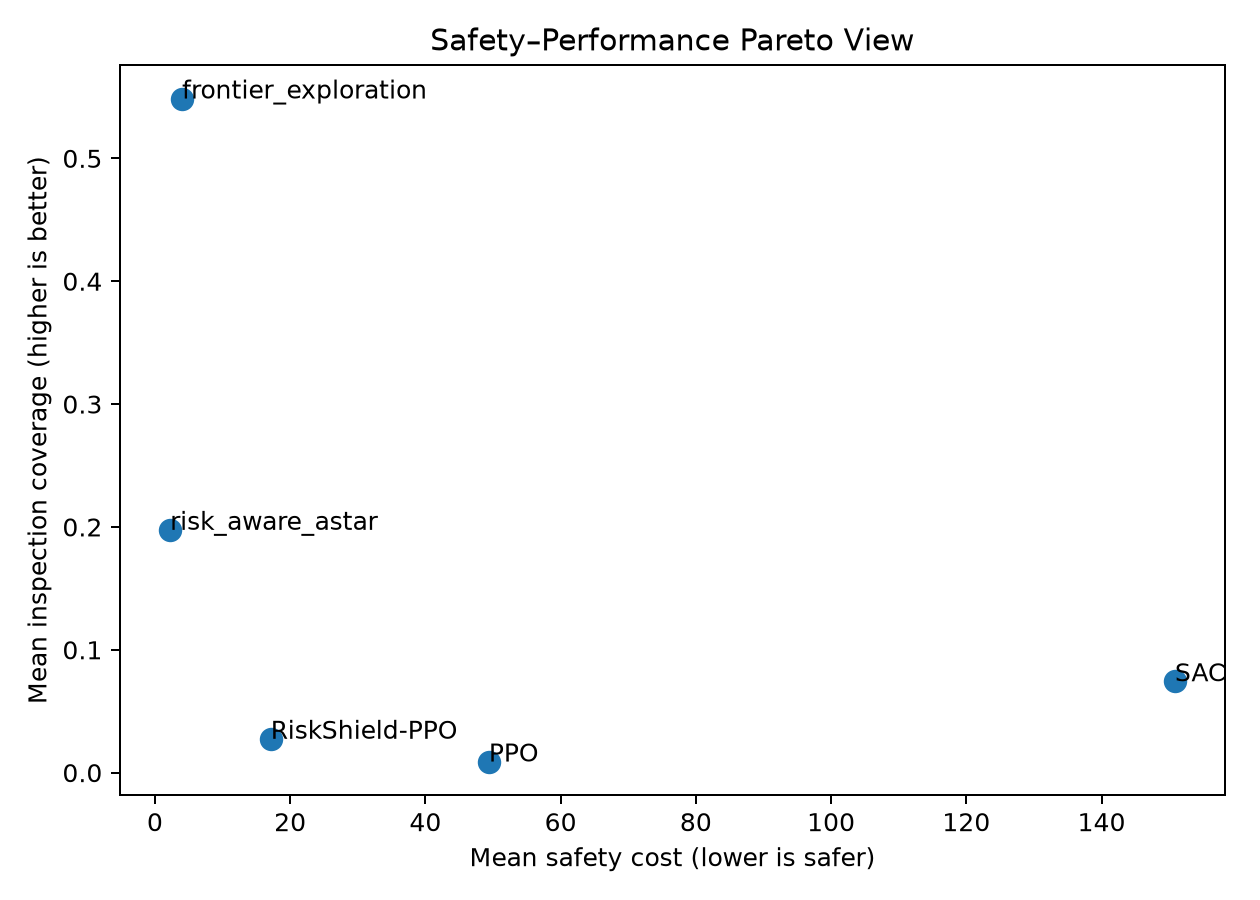
\includegraphics[width=\columnwidth]{figures/safety_performance_pareto.png}
\caption{Safety cost versus inspection coverage from raw primary records.}
\end{figure}

\section{Uncertainty Experiments}
False-negative probabilities are 0, 0.1, 0.2, and 0.3 in the dedicated
uncertainty suite. Lighting, blur, camera noise, moving-obstacle density, and
unseen layout are seeded. Clean truth, perturbed perception, and observation
are separate. Across 320 episodes and 64 conditions, mean robustness was
0.8893. Because baseline learned-policy mission success was zero, its ratio is
neutral rather than replaced by an invented improvement.

\begin{figure}[t]
\centering
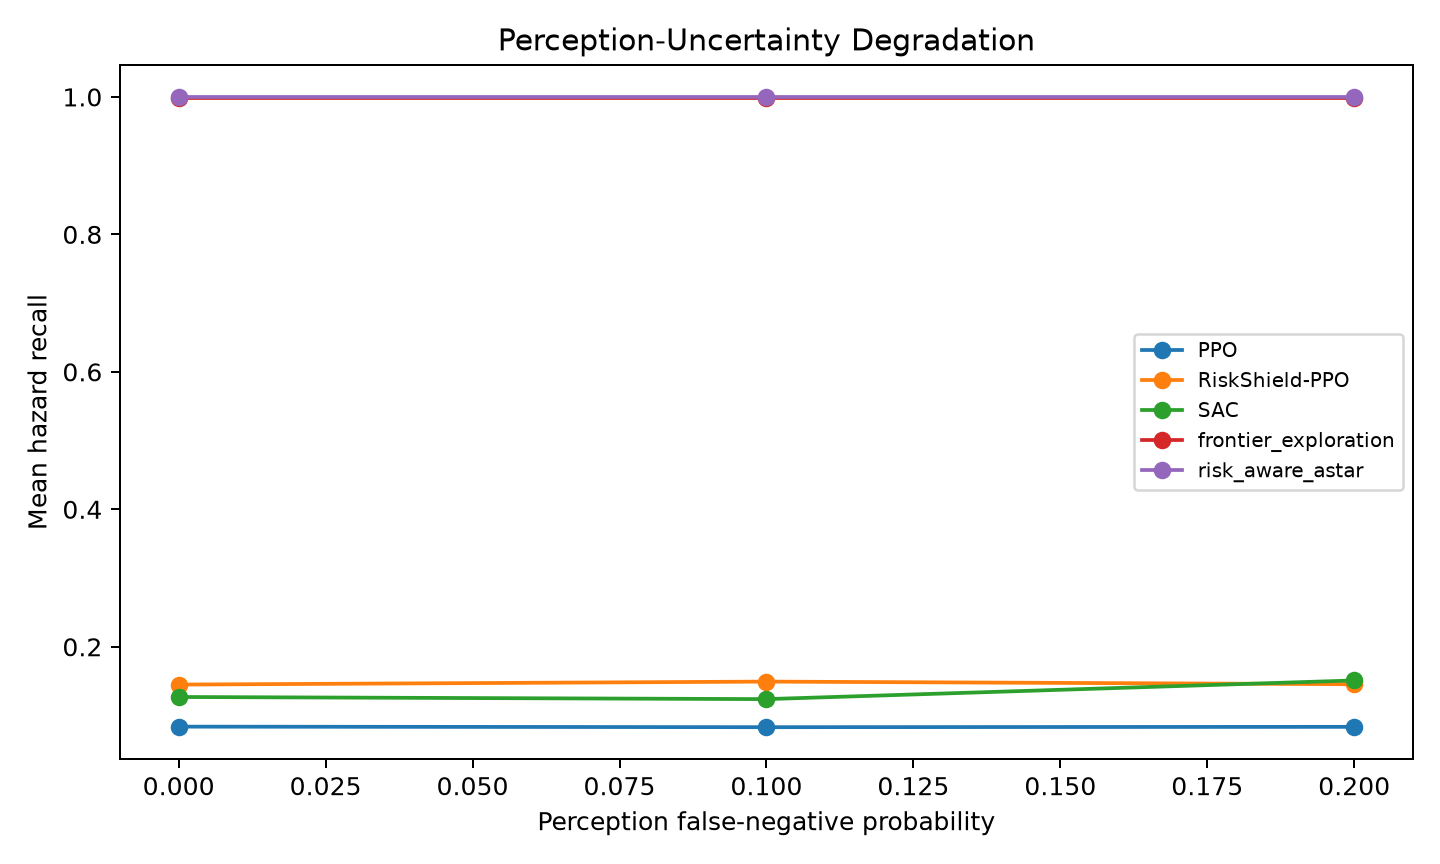
\includegraphics[width=\columnwidth]{figures/uncertainty_degradation.png}
\caption{Hazard-recall degradation derived from primary raw results.}
\end{figure}

\section{Ablation Study}
\begin{table*}[t]
\centering
\caption{Six paired ablations; 30 episodes per configuration.}
\resizebox{\textwidth}{!}{\begin{tabular}{lrrrrrr}
\toprule
Variant & Episodes & Recall & Coverage & Safety cost & Collision rate & Success \\
\midrule
One-step shield & 30 & 0.1661 & 0.0569 & 2.0667 & 0.0000 & 0.0000 \\
Full RiskShield-PPO & 30 & 0.1522 & 0.0408 & 8.4333 & 0.0000 & 0.0000 \\
Without action masking & 30 & 0.1211 & 0.0206 & 5.9000 & 0.0000 & 0.0000 \\
Without cost objective & 30 & 0.1522 & 0.0408 & 8.4333 & 0.0000 & 0.0000 \\
Without CV risk & 30 & 0.1522 & 0.0408 & 8.4333 & 0.0000 & 0.0000 \\
Without predictive shield & 30 & 0.1189 & 0.0291 & 66.5167 & 0.0000 & 0.0000 \\
\bottomrule
\end{tabular}
}
\end{table*}
Removing the predictive shield raised mean safety cost from 8.43 to 66.52.
The one-step shield produced lower cost (2.07) than $k=3$ in this limited
sample, so longer prediction was not uniformly better. Removing CV risk
injection or replacing the constrained checkpoint with PPO yielded identical
reported task means under the shield, although their internal actions and
intervention counts differed. This indicates that the shield dominated these
weak policies. Removing action masking reduced coverage.

\section{Discussion}
The planners' advantage indicates that exploration and long-horizon credit
assignment, not only collision avoidance, remain unsolved. RiskShield-PPO's
lower cost is meaningful but insufficient: a stationary or repeatedly
corrected policy can be safe and useless. The saturated multiplier suggests
the selected budget was difficult relative to the training distribution.
Future work should increase training budgets, tune cost scaling, evaluate
recurrent policies only after training a valid checkpoint, and separate shield
dependence from intrinsic policy safety.

\section{Limitations}
All research evaluation is simulation-only. Learned policies had zero complete
mission success. Stage 5C is a bounded integrated demonstration, not a
long-duration deployment. The detector supports only its recorded class list;
other semantic layers use simulator truth. No recurrent checkpoint exists, so
no recurrent ablation is claimed. Results cover one laptop GPU and Webots
R2025a. The shield is model-based and can fail under unmodeled dynamics. No
real-world safety guarantee, certification, or human-subject evaluation is
provided.

\section{Ethical and Safety Considerations}
The system must not replace qualified safety personnel or authorize entry into
hazardous areas. Simulator performance can create false confidence. Deployment
would require site-specific risk assessment, fail-safe hardware, independent
verification, privacy controls, worker consultation, and compliance with local
law and safety standards.

\section{Conclusion}
This work provides a reproducible construction Safe RL benchmark and truthful
evidence spanning planning, learned policies, constrained optimization,
shielding, uncertainty, CUDA perception, and Webots motor control.
RiskShield-PPO reduced cost but did not solve inspection; expert planners
remained substantially stronger. The negative result defines a clear research
target rather than a deployment claim.

\section*{Reproducibility Statement}
The repository records configuration files, seeds, checkpoint hashes, atomic
per-run caches, raw CSV and Parquet data, statistical scripts, figure source
data, tests, and PowerShell entry points. The complete benchmark command resumes
only missing runs. The production command separately reproduces the Webots
integration evidence.

\bibliographystyle{IEEEtran}
\bibliography{references}
\end{document}
